\section{Introduction}

Deliberation enables the generation, aggregation, and synthesis of diverse knowledge \cite{dewey_creative_1940, anderson_epistemology_2006, ackerman_deliberation_2002, ostrom_collective_2000},
as well as the early identification and resolution of conflict \cite{gentry_consensus_1982}.
As a participatory process, deliberation builds trust among participants, increases the perception of fairness, and incentivises cooperation with group decisions
\cite{ostrom_collective_2000, bowles_endogenous_1998}.
As a dynamic process, deliberation alters private preferences through discourse \cite{habermas_structural_1991}, sidestepping fundamental limitations of voting, e.g., the Condorcet paradox \cite{condorcet_essay_1785, brandt_computational_2012} and Arrow's impossibility theorem \cite{arrow_social_2012, brandt_computational_2012}.
Despite these benefits, deliberation becomes prohibitively difficult in larger groups, due to the increased time and effort needed to reach decisions \cite{fishkin_voice_1997, gentry_consensus_1982} and to the emergence of power inequalities \cite{freeman_tyranny_1972, boehm_egalitarian_1993}.
Yet examples of successful mass deliberation do exist, including Wikipedia \cite{giles_internet_2005, keegan_evolution_2017}, free and open source software projects \cite{benkler_coases_2002}, grassroots protest and crisis-response networks \cite{gonzalez-bailon_networked_2016, brugh_combining_2019} and self-managed organizations \cite{laloux_reinventing_2014}.
The commonalities between such projects provide insight into overcoming the challenges of mass deliberation.
Specifically, we evaluate a model of mass deliberation inspired by common network features observed in successful projects.

Communication in large collaborations is necessarily restricted when group size exceeds individual members' capacity for communication. The structure of the resulting communication network is an important factor in the success of collaborative tasks \cite{kearns_experiments_2012, mason_collaborative_2012, mason_propagation_2008}, such as deliberation. Among successful mass deliberative projects, communication networks often exhibits a common structure: small interlocking groups \cite{benkler_coases_2002, gonzalez-bailon_networked_2016, brugh_combining_2019, laloux_reinventing_2014}. A similar structure has been observed in the interlocking directorates of corporate boards \cite{karau_social_1993} and the interlocking publics of the public sphere \cite{habermas_structural_1991}, as well as utilized for collective design in network rotation \cite{salehi_hive_2018}.
These interlocking groups have been given various names: committees, working groups, projects, modules, affinity groups, circles, teams, cores, nodes, zones, cells, or syndicates.
We shall use the term {\em pods} to encompass all groups exhibiting two key characteristics: small enough to enable deliberation, and interlocking to enable information diffusion.
We shall use the term {\em network deliberation} to refer to mass deliberation using an interlocking pod structure.
Communication network structure also influences the success of collaborations by controlling the speed of information diffusion \cite{lazer_network_2007,mason_propagation_2008,mason_collaborative_2012,barkoczi_social_2016, gomez_clustering_2019,derex_partial_2016,kearns_experiments_2012}. Structurally efficient networks enable fast diffusion and favor exploitation of known information over exploration of the unknown \cite{lazer_network_2007, barkoczi_social_2016}. In the context of network deliberation, structural efficiency is determined by how individuals are assigned to pods.
We will focus on two such methods: one efficient, one inefficient.

Collective tasks such as deliberation are influenced not only by communication structure, but also by individual behavior. Individuals weigh social influence against their personal knowledge and expertise  \cite{boyd_culture_1988}. 
Even in a collective setting, individuals sometimes work independently to search for new and innovative ideas \cite{lazer_network_2007, barkoczi_social_2016}, to utilize their unique information and perspectives \cite{hong_interpreted_2009}, and to critically evaluate the ideas of others \cite{rendell_rogersparadox_2010}.
Alternatively, individuals can defer to others in order to exploit and propagate good ideas \cite{barkoczi_social_2016, boyd_culture_1988}, to conserve their own resources through free-riding and social loafing \cite{karau_social_1993}, or due to a high level of trust \cite{salehi_hive_2018} or social influence \cite{banerjee_simple_1992, smith_pathological_2000}. Individual behavior interacts with network structure to vary the level of exploration of new ideas versus the exploitation of known information \cite{barkoczi_social_2016}. While the focus of network deliberation is structural, the effect of network structure must be understood in the context of individual behavior and social dynamics.

We model network deliberation using a social learning framework to address two questions. How effective is network deliberation compared to conventional single-group deliberation? And how do network efficiency and individual behavior influence the outcome of network deliberation? We present the following three contributions.
First, network deliberation out-performs conventional deliberation in both solution speed and quality when agents rely heavily on social learning. This suggests that network deliberation is a promising deliberation design for groups with a high degree of social influence. Second, network deliberation performs best on structurally efficient networks when agents exhibit conformist behavior, while it performs best on structurally inefficient networks when agents greedily maximize solution quality, consistent with findings for conventional networks \cite{barkoczi_social_2016}.
Third, the naive greedy strategy can be modified to improve performance on conventional networks despite using strictly less information. In the case of network deliberation, the naive and modified greedy strategies are equivalent.

\section{Methods}

Deliberation can be modeled as a form of collective problem-solving and social learning in which agents hold private beliefs, share information with their neighbors, and update their beliefs based on a combination of individual analysis and social influence.
Following existing models of collective problem-solving \cite{lazer_network_2007, barkoczi_social_2016, gomez_clustering_2019}, our model comprises: 1. a collective task, 2. a network, and 3. a learning strategy.
Agents maintain a candidate solution to the task and iteratively apply their learning strategy to the available information, yielding an updated candidate.

\subsection{Overview}

As their collective task, agents seek an optimal point on a rugged fitness landscape.
This landscape is generated using the NK model \cite{kauffman_towards_1987, weinberger_local_1991} (see Appendix \ref{apx-nk}).
The NK model is a ``tuanbly rugged'' objective function parameterized by two variables:
the number of bits in the input string ($N$),
and the number bits used to compute each contribution to the objective function ($K+1$).
These parameters can be used to tune problem size and complexity, respectively.
The resulting objective function maps $N$-bit strings to real numbers in $[0,1]$.

To model network deliberation, we construct interlocking networks in stages. At each stage, agents are partitioned into small {\em pods} and connected to all other agents in the same pod.
Our choice of pod size is informed by real-world The upper limit of effective small group size has been estimated variously as five \cite{freeman_tyranny_1972}, five--eight\cite{lohman_designing_2000}, and eight \cite{miflin_small_2004}.
We choose a pod size of 5.
Different methods for assigning agents to pods produce networks with different properties.
Interlocking structure is created when agents are placed with others they have not yet interacted with.
We thus require that pod assignment methods satisfy the following mixing property:
\begin{property}
\label{prop:mixing}
For any agent $v$, and any two assignment stages $t$, $t^\prime$, the probability that at least one neighbor of $v$ at stage $t$ is also a neighbor at stage $t^\prime$ approaches 0 as $|V|$ grows.
\end{property}
We study two such methods: a random assignment method that produces structurally efficient networks, and a long-path method that produces inefficient networks. For comparison, we also simulate conventional deliberation. While the potential communication links in conventional deliberation form a fully connected network, actual communication is better modeled by preferential attachment \cite{barabasi_emergence_1999} or small-world \cite{watts_collective_1998} networks (see Methods).

An agent's learning strategy models both informational constraints and behavioral dynamics \cite{lazer_network_2007, barkoczi_social_2016} such as social influence and social loafing \cite{karau_social_1993}.
We consider three social learning strategies.
The {\em best-neighbor} strategy is the naive greedy strategy: agents simply adopt the neighboring solution with the highest value. This strategy requires that agents have the ability to compare the quality of two arbitrary solutions, a strong assumption representing either skilled agents, or a simple task.
The {\em conform} strategy is pure social influence. Agents adopt the most common solution among their neighbors.
This strategy requires no knowledge of solution quality, modeling contexts where agents are unable to compare solution quality, or where agents choose not to, as in social loafing \cite{karau_social_1993}.
We also introduce the {\em confident-neighbor} strategy, a variant of best-neighbor in which agents announce when they have the best solution in their neighborhood. This variant makes weaker assumptions about agent ability but is equivalent to best-neighbor when network deliberation is used.
This strategy allows us to compare low-social influence and high-social influence strategies under equivalent assumptions of agent ability.

Between each stage of social learning, agents may perform individual learning. Following existing literature \cite{lazer_network_2007, barkoczi_social_2016}, we model individual learning by mutating a single bit of an agent's solution, and keeping it if the mutation improves solution quality.
A complete learning strategy must also specify how social and individual learning are integrated. Existing literature \cite{lazer_network_2007, barkoczi_social_2016} applies individual learning only when social learning fails to produce an improved solution. We refer to this method as {\em fallback} individual learning. Fallback can be also be interpreted as a model of social loafing \cite{karau_social_1993}. For completeness, we include analysis for a second method in which agents first perform social and individual learning in {\em parallel} and then choose the better of the two learning outputs.

\subsection{Agent-Based Model}

We use an agent-based simualation to model deliberation between individuals.
We model communication between agents using a time-dependent network $(V,E_t)$.
The vertices $V$ correspond to the agents (individuals).
The edges $E_t$ allow agents to exchange information with their immediate neighbors at time $t$.
Over the course of the simulation, agents seek to maximize some objective function $Q(s)$.
We use binary strings of length $d$ as our solution space: $s \in \mathbb{Z}^d$.
We generate the objective function $Q(s)$ using the NK model \cite{kauffman_towards_1987, weinberger_local_1991} (see Appendix \ref{apx-nk}).

The simulation begins at time $t=0$ by generating a set of initial solutions $s_{v,0}$ for the agents.
These are generated randomly, with each possible solution having equal probability.
The simulation proceeds iteratively.
At time $t$ each agent applies one of several {\em learning strategies}, to determine its preferred solution at time $t+1$.
Learning strategies can rely on the agent's own solution, the solutions of its neighbors, and potentially additional information shared by its neighbors.
Learning strategies may also incorporate information about the objective function, modeling an agents' ability to evaluate the quality of solutions.
To allow for ties, learning strategies produce a set of solutions rather than a single solution.
In our simulations, we choose winners at random in the case of a tie.
We present results for 1000 randomly generated NK model objectives.
with each network/strategy combination simulated once per objective function.
In keeping with other authors \cite{barkoczi_social_2016, lazer_network_2007} we use $N=15$ and $K=6$.
We allow each simulation to proceed for 300 iterations, which we have found sufficient to guarantee convergence with our chosen parameters.

\subsection{Networks}

We carry out simulations for four different network topologies. In addition to the well-known preferential-attachment \cite{barabasi_emergence_1999} and small-world \cite{watts_collective_1998} networks, we construct two types of networks to model network deliberation.
Both types exhibit interlocking structure and satisfy Property \ref{prop:mixing}.
These two network deliberation conditions differ in how agents are assigned to pods and in the structural efficiency of the resulting network.
At each iteration, existing edges are replaced with cliques corresponding to the pods. An edge is created between two agents if and only if they share a pod.
In {\em random-pod} assignment, agents are assigned to pods at random.
This assignment method produces short geodesic paths and efficient network structure.
In {\em long-path} assignment, agents are assigned using an algorithm which guarantees interlocking structure while preventing the creation of long-distance ``shortcut'' edges, producing a structurally inefficient network.
All networks are constructed with 100 vertices/agents and a mean degree of 4 (pod size of 5).

\subsection{Conventional Deliberation}
We model the communication network structure of conventional deliberation using two static networks: small-world networks \cite{watts_collective_1998}, and preferential attachment networks \cite{barabasi_emergence_1999}. In typical deliberative settings, from deliberative assemblies to online forum threads, the contributions of any member are potentially visible to all other members.
The network of {\em potential} communication can be modelled by a complete graph.
However, a complete graph may not be the best model for the {\em actual} communication that takes place in such a network. In a real-world deliberation, some participants are more influential than others \cite{goel_structure_2012, shaw_laboratories_2014}, and many communications can be missed or ignored by any particular participant.

Human social networks often exhibit large clustering, and short path lengths.
To model such dynamics, we use Watts-Strogatz small-world networks  \cite{watts_collective_1998}.
These networks model, for example, when participants interact mostly with their strong ties, but occasionally with a weak tie. Social networks have also been found to exhibit skewed degree distributions with long tails \cite{barabasi_emergence_1999}.
We model these networks using the Barabási-Albert preferential attachment model.
These networks model settings where a small number of individuals produce a disproportionate share of the communication due to factors such as social capital, expertise, or confidence.

\subsection{Network Deliberation: Interlock Networks}
Both of our network deliberation conditions use networks built from interlocking pods.
These pods are small complete graphs of roughly equal size.
At any given time, each agent can communicate with all other agents in exactly one pod.
Periodically, all agents are simultaneously reassigned to new pods.
These reassignments create an interlocking structure, allowing information to flow through the entire group.
This structure can be represented as a time-dependent or directed network.
The properties of an interlock network depend on the particular method for assigning agents to pods.
Crucially, interlocking structure is created when agents are placed with others they have not yet interacted with.
We thus require that pod assignment schemes satisfy the mixing property (Property \ref{prop:mixing}).

\subsubsection{Random-Pod Assignment}
The {\em random-pod} assignment method (Algorithm \ref{alg:random}) simply assigns agents to groups at random. Pseudocode for this method is shown in Algorithm \ref{alg:random}.

\begin{algorithm}
\SetAlgoLined
\DontPrintSemicolon
\SetKwFunction{removeRandom}{removeRandom}
\SetKwFunction{insert}{insert}
\SetKwFunction{emp}{empty}
\SetKw{algnot}{not}
\KwData{A vertex list $V$, the pod size $M \in \mathbb{Z}$.}
\KwResult{A partition of the vertices.}
    $N \longleftarrow \lceil \frac{|V|}{M} \rceil$ \;
    $P \longleftarrow$ List of $N$ empty sets \;
    \For{$i \in 1, \ldots, M$}{
        \ForEach{$s \in P$}{
            \If{\algnot $V.\emp()$}{
                $v \longleftarrow V.\removeRandom()$ \;
                $s.\insert(v)$ \;
            }
        }
    }
    \Return{$P$}
\caption{Random-Pod Assignment}
\label{alg:random}
\end{algorithm}

\begin{claim}
Random-pod assignment satisfies Property \ref{prop:mixing}.
\end{claim}

\begin{proof}
Let $v$ be a vertex of graph $G=(V,E_t)$ with a set of $M$ neighbors at stage $t$ denoted $N_t(v)$.
The probability that the $k$th neighbor chosen at time $t^\prime \neq t$ belongs to $N_t(v)$, given that the first $k - 1$ did not, is:
\begin{align*}
p_\text{repeat}(k)
&= \frac{M - 1}{|V| - k} \\
&\leq \frac{M - 1}{|V| - M}.
\end{align*}
The probability that none of the $M-1$ neighbors chosen at time $t^\prime$ belong to $N(v)$ thus satisfies:
\begin{align*}
p_\text{mixed}
&\geq
\left( 1 - \frac{M - 1}{|V| - M} \right)^{M-1} \\
\lim_{|V|\rightarrow\infty} p_\text{mixed}
&= 1
&\qedhere
\end{align*}
\end{proof}

Random pod assignment also creates structurally efficient networks with short geodesic distances, as shown in Figure \ref{fig:broadcast}.
There has been evidence both for
\cite{lazer_network_2007, derex_partial_2016, mason_propagation_2008, barkoczi_social_2016}
and against
\cite{mason_collaborative_2012, barkoczi_social_2016}
the effectiveness of structurally efficient networks in social learning.

\begin{figure}
    \centering
    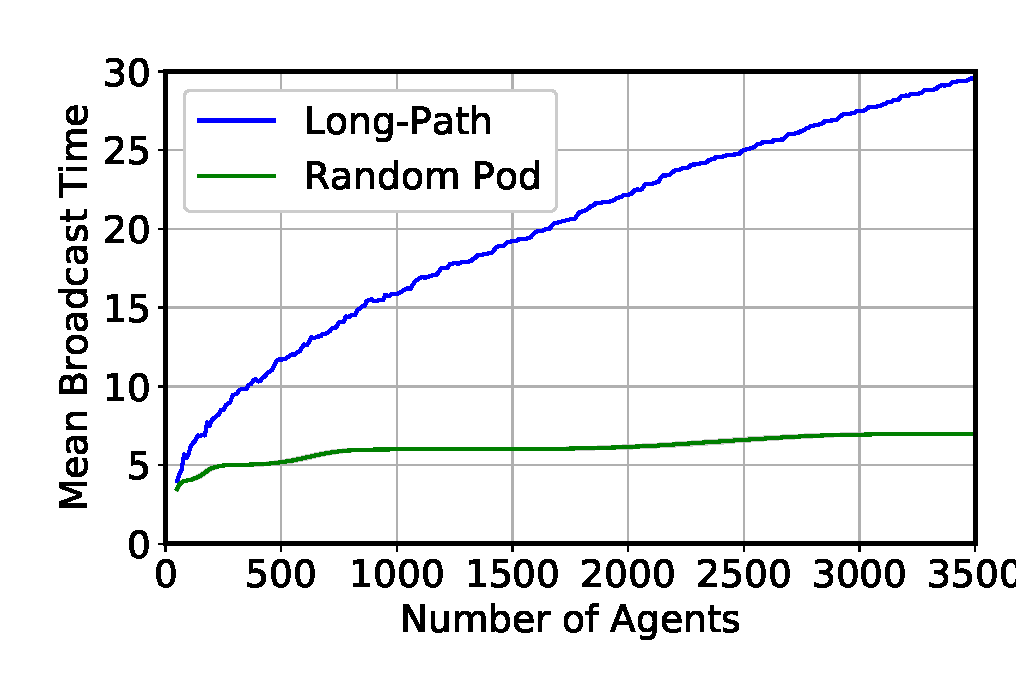
\includegraphics[width=3.33in]{fig/NetDelibABM/fig-broadcast.eps}
    \caption{Mean time necessary for a signal broadcast from one node to reach the entire network. We use mean broadcast time as a measure of geodesic length for time-varying networks.}
    \label{fig:broadcast}
\end{figure}


\subsubsection{Long-Path Pod Assignment}

To study the effects of path length, we require an alternative pod assignment method that produces long paths.
However, we must still retain Property \ref{prop:mixing} such that it is rare for two agents to repeatedly share the same pod.
This property ensures the creation of many new edges at each stage, which is difficult--but not impossible--to reconcile with long average path length.
We now present a {\em long-path} pod assignment method, which meets both of the above goals.

We begin with a high-level overview.
Agents are assigned an integer position on a 1-dimensional circular lattice.
By preferring short-distance links on this lattice, we maintain long path lengths.
We also partition agents according to the remainder of their position, modulo some prime, i.e., their residue class.
By limiting links to agents in the same residue class, and using a unique prime at each stage, we ensure that it is rare for multiple agents to share a pod twice in a row.
Specifically, for stages using primes $p$ and $q$, two agents will share a pod for both stages when their positions are equal modulo $pq$. Pseudocode for long-path assignment is shown in Algorithm \ref{alg:long}.

\begin{algorithm}
\SetAlgoLined
\DontPrintSemicolon
\SetKw{algnot}{not}
\SetKwFunction{removeRandom}{removeRandom}
\SetKwFunction{moduli}{moduli}
\SetKwFunction{append}{append}
\SetKwFunction{enqueue}{enqueue}
\SetKwFunction{dequeue}{dequeue}
\SetKwFunction{concat}{concatenate}
\KwData{A vertex list $V$, the pod size $M \in \mathbb{Z}$, the stage $t \geq 0 \in \mathbb{Z}$, a list of co-prime integers $\moduli$.}
\KwResult{A partition of the vertices.}
    $N \longleftarrow \lceil \frac{|V|}{M} \rceil$ \;
    $P \longleftarrow$ List of $N$ empty sets \;
    \eIf{$t = 0$}{
        // Place all vertices in same residue class \;
        $p \longleftarrow 1$ \;
    }{
        // Choose integer to define residue class \;
        $p \longleftarrow \moduli[t]$ \;
    }
    // Assign vertices to residue classes \;
    $R \longleftarrow$ List of $p$ empty queues \;     
    \For{$z \in 0, \ldots, |V|-1$}{
        $R[z \bmod p].\enqueue(V[z])$ \;
    }
    // Divide each residue class into pods \;
    $P \longleftarrow $ Empty list of lists. \;
    \For{$r \in R$}{
        $N_r \longleftarrow \lceil \frac{|r|}{M} \rceil$ \;
        $P_r \longleftarrow$ List of $N_r$ empty lists \;
        \For{$i \in 1, \ldots, M$}{
            \For {$j \in 0, \ldots, N_r - 1$}{
                \If{ \algnot $r.\emp()$}{
                    $v \leftarrow r.\dequeue()$ \;
                    $P_r[j].\append(v)$ \;
                }
            }
        }
        $P.\concat(P_r)$
    }
    \Return{$P$}
\caption{Long-Path Assignment}
\label{alg:long}
\end{algorithm}


\begin{claim}
When the pod size $M$ is less than the modulus $p_t$ for all stages $t$, long-path pod assignment satisfies Property \ref{prop:mixing}.
\end{claim}

\begin{proof}
Let $p$ and $q$ be co-prime integers used as moduli for stages $t$ and $t^\prime$ respectively.
Let $z(x)$ denote the integer position of vertex $x$.
Let $v$ be a vertex, and let us assume vertex $w$ belongs to the same pod as $v$ at both time $t$ and $t^\prime$.
This assumption implies:
\begin{align*}
    z(v) &\equiv z(w) \pmod{p} \\
    z(v) &\equiv z(w) \pmod{q} \\
    \implies z(v) - z(w) &\equiv 0 \pmod{p} \\
    &\equiv 0 \pmod{q} \\
    &= npq & \text{for some integer n}.
\end{align*}
By the definition of the long-path algorithm:
\begin{align*}
    |z(v)-z(w)| & \leq (M - 1)p \\
    \implies |n|pq & \leq (M - 1)p \\
    |n|q & \leq (M - 1).
\end{align*}
By assumption, $q \geq M$, so the above can only be satisfied by $n=0$,
which in turn implies $v=w$. \qedhere
\end{proof}

To see that the long-path procedure produces long geodesics, note that the pods of size $M$ connect nodes at most $(M - 1)p_i$ apart in position, preventing the creation of any shortcut edges, as long as $p_i$ is small compared to $|V|$.
Numerical simulations confirm that the long-path algorithm produces geodesics larger than random pod assignment (Figure \ref{fig:broadcast}).
The number of agents may not be an exact multiple of $M$, so the final pods may be truncated. However, the network will be a sub-graph of a network that does have a multiple of $M$ nodes, so the structure will not be fundamentally changed, and these edge effects should become negligible as the number of agents increases.


\subsection{Learning Strategies}
We simulate three learning strategies. Each strategy combines an individual strategy and a social strategy. The individual strategy is the same for all conditions. Agents chose a random bit of their current solution and invert that bit. If the resulting solution is an improvement, it is kept, otherwise the original is kept.
We simulate two methods of combining individual and social strategies. In the {\em fallback} condition, individual learning is only applied when social learning fails to improve the solution.
In the {\em parallel} condition, individual and social strategies are applied to the original solution in parallel and the better of the two is chosen. In all cases, a final check is performed, following \cite{barkoczi_social_2016}: new solutions are only accepted if they improve on the original solution. Descriptions of the social learning strategies follow (formal definitions can be found in the Supplementary Information).

The {\em best-neighbor} strategy closely follows that used by other authors \cite{lazer_network_2007, barkoczi_social_2016}. To apply this strategy, an agent searches the solutions of all immediate neighbors, and chooses the solution maximizing the payoff. In the event of a tie, one of the maximal solutions is chosen at random, with probability proportional to the number of neighbors exhibiting that solution.

The {\em conform} strategy also follows previous authors \cite{barkoczi_social_2016}. To apply this strategy, agents search the solutions of all immediate neighbors, counting the number of times each unique solution appears. The solution with the highest count is adopted. In the event of a tie, the original solution is maintained.

The {\em confident-neighbor} strategy is a novel variant of best-neighbor. To apply this strategy, agents search the solutions of all immediate neighbors to determine if any are superior to their own. If no superior solutions are found, the agent is {\em confident}. The confident agent maintains its original solution and broadcasts that solution to all neighbors. Alternatively, if superior solutions are found, the agent waits for broadcasts from confident neighbors. Agents may receive zero, one, or many such broadcasts. If no broadcasts are received, the agent maintains its original solution. If one or more broadcasts are received, one of them is chosen at random and that solution is adopted. It is worth noting that this strategy is equivalent to best-neighbor when the network is composed of one or more cliques, as in network deliberation.

\subsection{Statistical Methods}
All comparisons are made using two-tailed paired t-tests. Pairs of observations correspond to the same instance of the NK-model objective function.
Significance values have been corrected for multiple comparisons using the Bonferroni correction.

\section{Results}

Here we present the results of 1000 runs of an agent-based model of deliberation.
In each run, an NK model is generated (N=15, K=6) and the model is simulated for 300
iterations for each network/strategy combination.
The results of these simulations are shown in Figure \ref{fig:results}.

We find that network deliberation identifies higher quality solutions than
conventional deliberation when agents use the conform strategy,
while requiring less time to converge. Within network deliberation,
we find that the structurally efficient random pod network outperforms the
structurally inefficient long-path network when agents use the conform strategy.
However, when either best-neighbor or confident-neighbor is used,
the inefficient network is preferable, consistent with findings for conventional
networks \cite{barkoczi_social_2016}. We also find that the confident-neighbor
strategy matches or outperforms best-neighbor across all networks,
despite using strictly less information about solution quality.

\begin{figure*}[]
    \label{fig:results}
    \centering
    \begin{minipage}{3.33in}
        \centering
        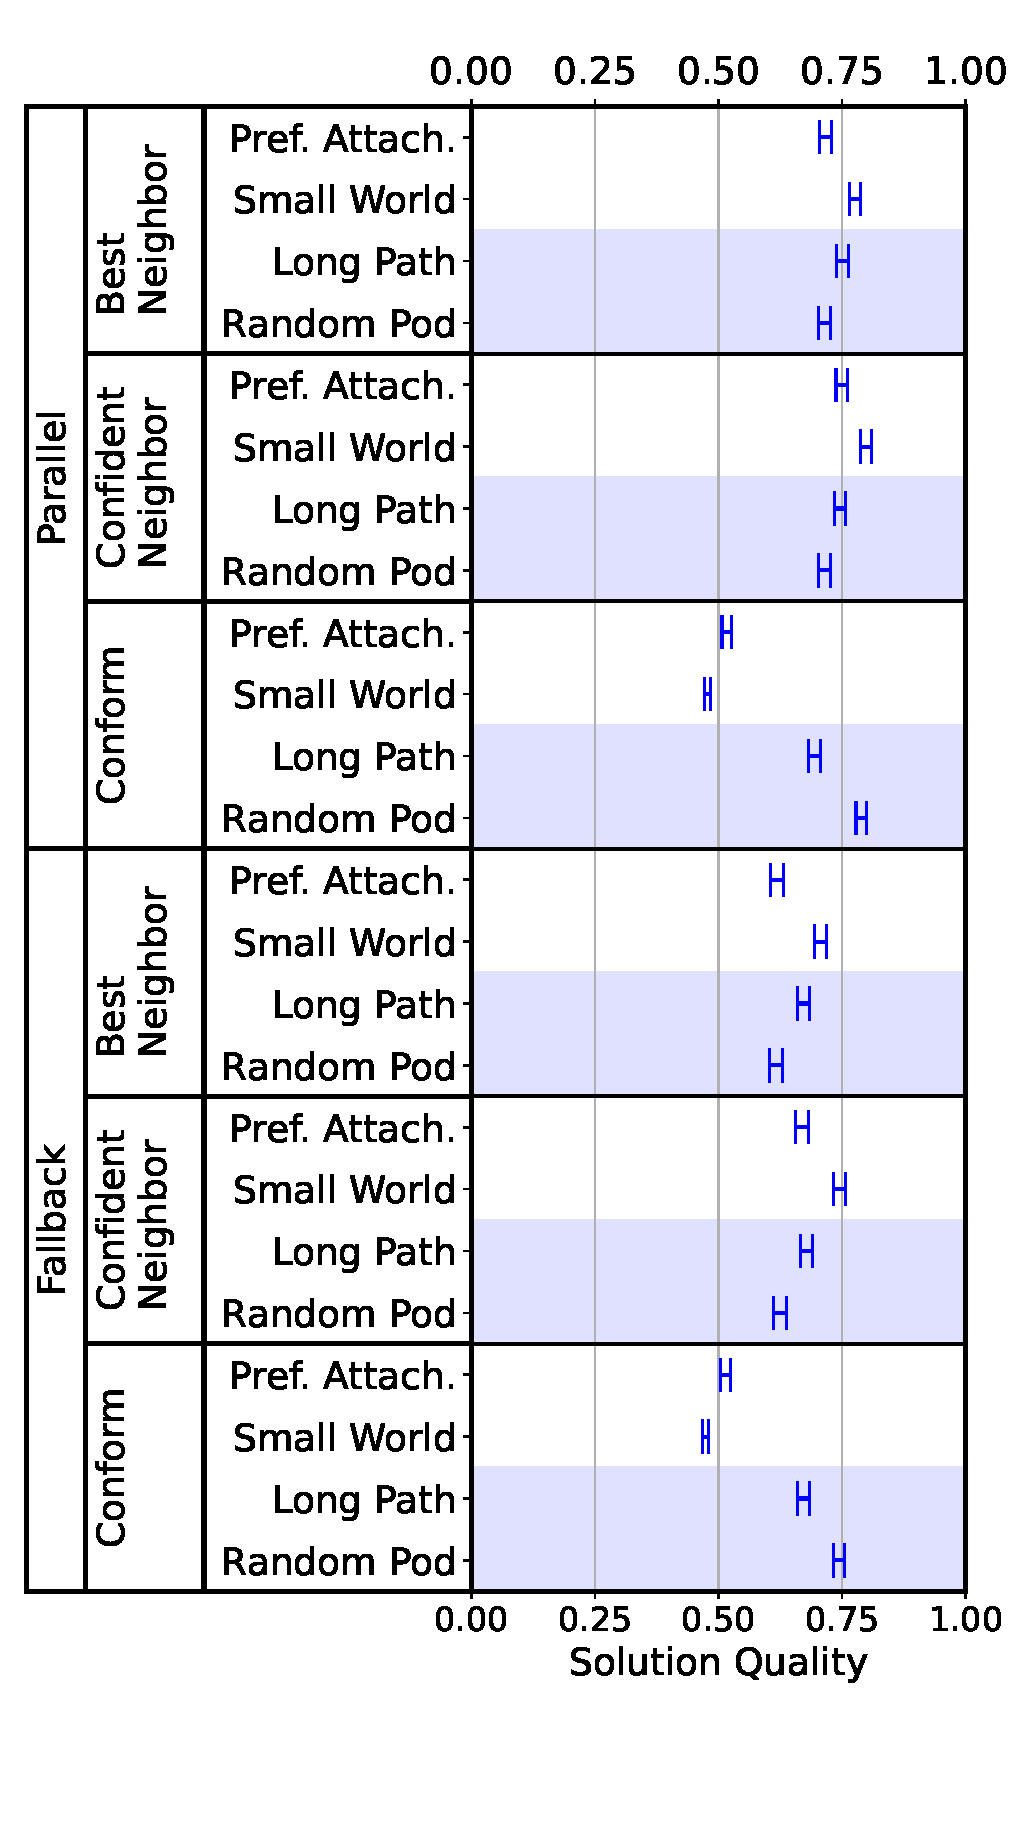
\includegraphics[width=3.33in]{fig/NetDelibABM/fig-perf-both.eps}
    \end{minipage}%
    \begin{minipage}{1.875in}
    \centering
    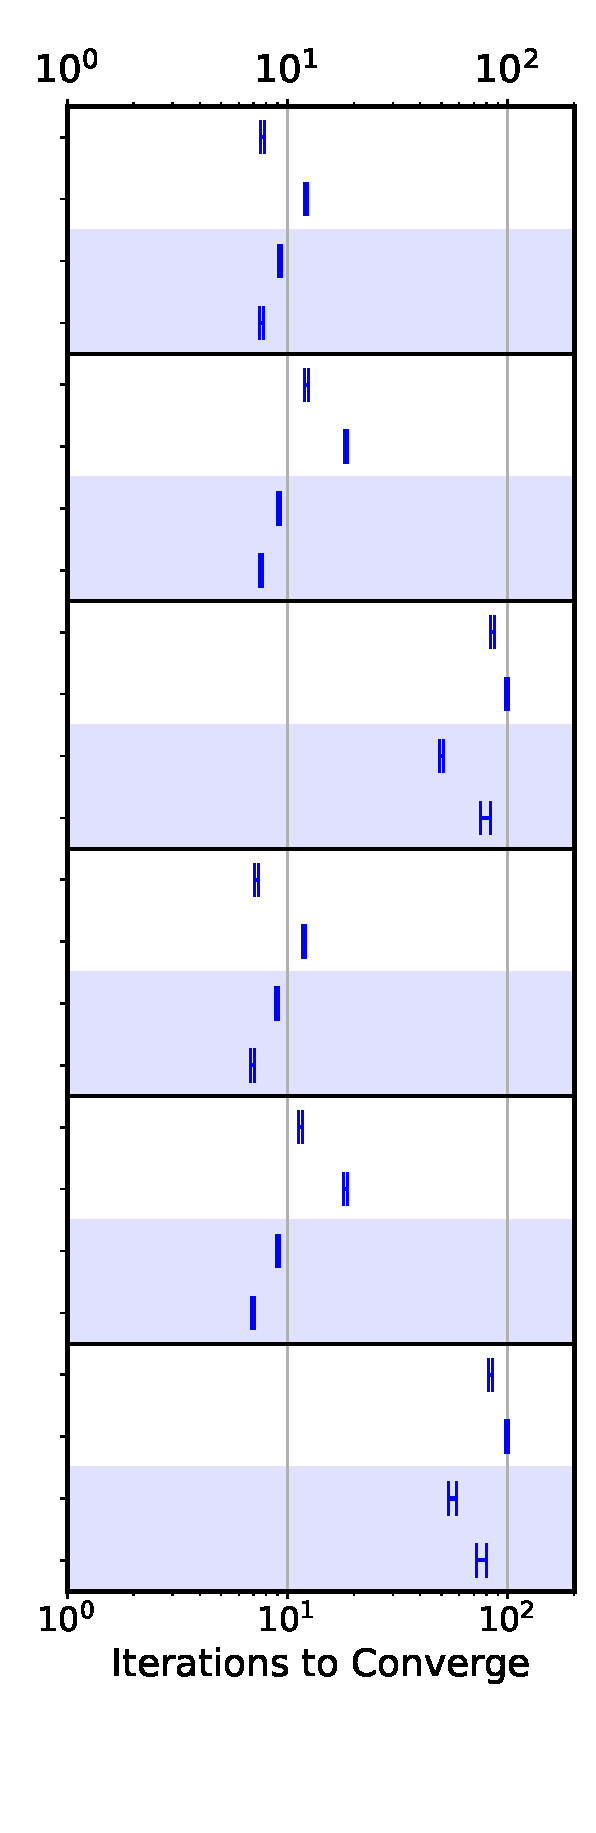
\includegraphics[width=1.875in]{fig/NetDelibABM/fig-converge-both.eps}
    \end{minipage}
\caption{
Solution quality and convergence time for agent-based simulations of different learning strategies. Error bars represent 95\% confidence interval. Results for network deliberation are shown shaded.
}
\end{figure*}

\subsection{Network vs. Conventional Deliberation}
We are particularly interested in comparing the performance of network deliberation to that of conventional single-group deliberation. When the conform strategy is used, we find that both of the network deliberation conditions yield better performance than conventional networks (Figure \ref{fig:results-conform-diff}). Analysis of the solution quality distributions (Figure \ref{fig:results-conform-dist}) shows two distinct effects. First, network deliberation frequently finds maximal solutions while conventional deliberation does not. Second, even when non-maximal solutions are found, network deliberation finds higher-quality solutions. This benefit is robust across both parallel and fallback individual learning. The effect size is dramatic. Conventional networks combined with the conform strategy show the lowest performance of all conditions, while random pod network deliberation combined with the conform strategy shows higher performance than nearly all other conditions. The exception being small world network combined with the best/confident-neighbor strategy, which shows equal performance within our statistical resolution. 
Often, increased performance comes at the expense of speed as more time is devoted to exploring novel solutions. However, we find that network deliberation improves both performance and speed when the conform strategy is used, suggesting that interlocking network structure can enable more efficient exploration.

\begin{figure}
    \label{fig:results-conform-diff}
    \centering
    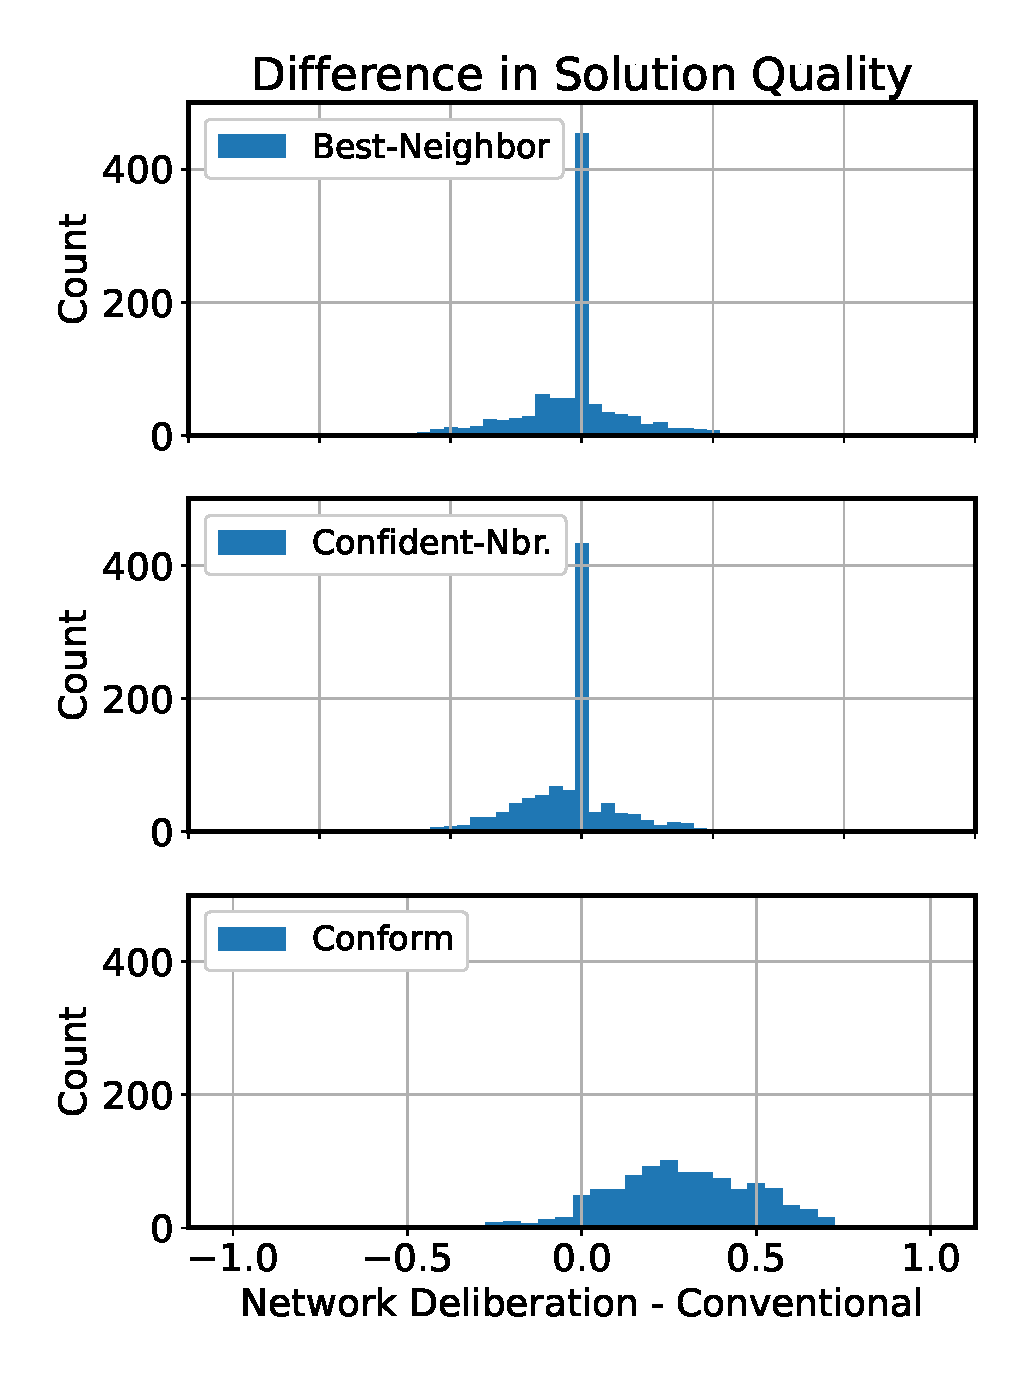
\includegraphics[width=3.33in]{fig/NetDelibABM/fig-results-netdelib-diff.eps}
\caption{Difference in solution quality between network deliberation and conventional deliberation. Plots for Best/Confident-Neighbor show results for long-path and small-world networks, while the plot for conform shows results for random-pod and preferential-attachment networks. Results are shown for parallel individual learning.}
\end{figure}

\begin{figure}
    \label{fig:results-conform-dist}
    \centering
    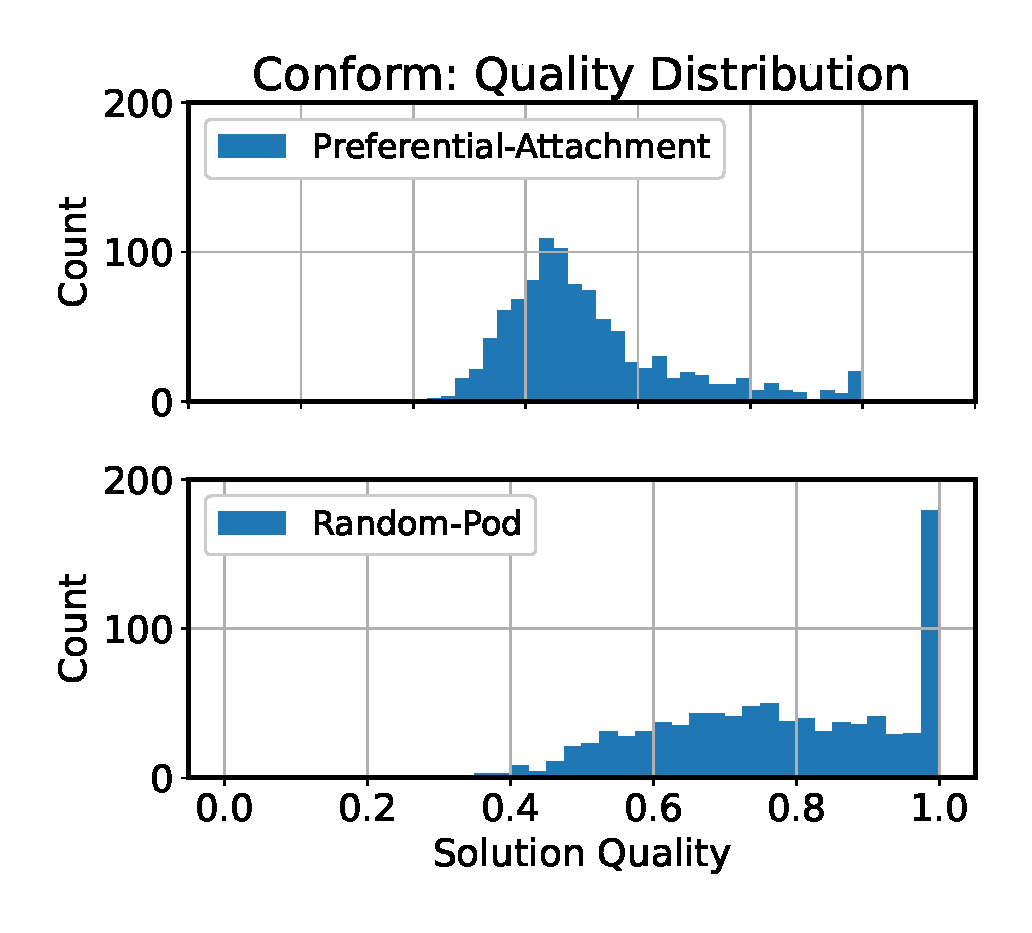
\includegraphics[width=3.33in]{fig/NetDelibABM/fig-results-conform-dist.eps}
\caption{Distributions of solution quality for social learning on a preferential-attachment network and random-pod network deliberation. Results are shown for parallel individual learning.}
\end{figure}

The conform strategy models contexts in which individuals rely heavily on social influence. Such contexts can arise from pro-conformity social norms, high levels of trust, social loafing, and limited information. As a form of rational ignorance, conformist behavior can conserve individual resources, but poses the risk of forming information cascades and propagating misinformation and inferior or harmful innovations \cite{banerjee_simple_1992}. Our simulations show that network deliberation can greatly improve the outcome of deliberation in the presence of strong social influence. This insight suggests one possible mechanism behind the success of mass deliberative projects, as well as the potential for network-based interventions in mass deliberation.

\subsection{Structural Efficiency}

The speed at which information can move through a communication network, i.e., it's structural efficiency, has been found to influence the success of collective problem-solving. We might expect the same to be true in network deliberation. In network deliberation, network structure is created through group membership. We compare the results of two group assignment methods: a random pod assignment yielding an efficient network, and a long-path method yielding a less efficient network (Figure \ref{fig:results-netdelib-efficiency}). We find that for greedy strategies (best-neighbor and confident-neighbor), the inefficient network yields the better results. The results are opposite for the conform strategy, with the efficient network yielding better results. These results are consistent with those observed for conventional single-group networks \cite{barkoczi_social_2016}, but to the best of our knowledge, they had not been explored for interlocking network like the ones we use to model network deliberation.

\begin{figure}
    \label{fig:results-netdelib-efficiency}
    \centering
    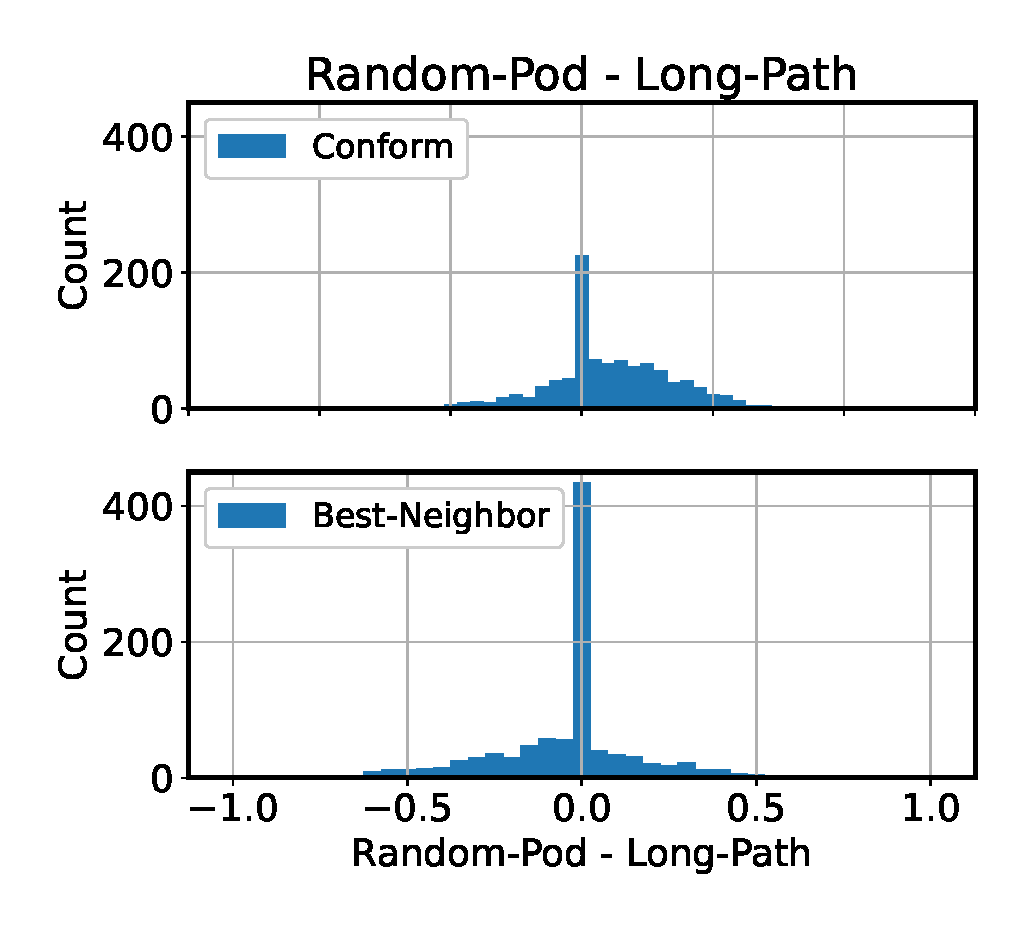
\includegraphics[width=3.33in]{fig/NetDelibABM/fig-results-netdelib-efficiency.eps}
\caption{Difference in solution quality between random-pod (efficient) and long-path (inefficient) network. Results are shown for parallel individual learning.}
\end{figure}

The role of structural efficiency in collective tasks can be partially attributed to diversity \cite{lazer_network_2007, hong_groups_2004}. Greedy strategies such as best/confident-neighbor result in agents adopting the highest quality solution they have seen so far and discarding all others. Such strategies quickly reduce the number of solutions present in the population, quickly identifying a local maximum at the cost of diversity. As a result, agents duplicate efforts during individual learning, exploring mutations of the same solution. Inefficient networks can mitigate this effect by slowing the spread of high-quality solutions and allowing time for the exploration of new and potentially better solutions. Our results show exactly this, with long-path pod assignment improving the performance of greedy algorithms. The improved performance of the conform strategy in random pod assignment can be attributed to the converse of the above. When social influence is strong, efficient networks can interrupt information cascades by introducing new information from far across the network.
Our results are thus generally consistent with existing theory on structural efficiency and collective problem-solving.
However, we note an interesting deviation: under the conform strategy, long-path network deliberation out-performs the two conventional networks, both of which are more efficient.

\subsection{Confident-Neighbor Strategy}

In general, the best-neighbor strategy requires strong assumptions about agents' ability to evaluate solutions. In the special case of network deliberation, the assumptions can be weakened by applying a variant of the strategy, which has not been previously studied. The variant, which we call {\em confident-neighbor}, is equivalent to best-neighbor for network deliberation, but not in general. Confident-neighbor thus provides a comparison between network deliberation and conventional single-group deliberation under weaker informational assumptions than best-neighbor. Surprisingly, the weaker assumptions of confident-neighbor lead to higher performance on the preferential attachment network, and similar performance on the-small world network (within our statistical resolution). Figure \ref{fig:results-confident} shows histograms of the quality difference between confident-neighbor and best-neighbor for both conventional networks. In the majority of cases, both strategies find comparable solutions. However, we find that when these strategies do find different solutions, those found by confident-neighbor are more often better, at least for the preferential-attachment network.

\begin{figure}
    \label{fig:results-confident}
    \centering
    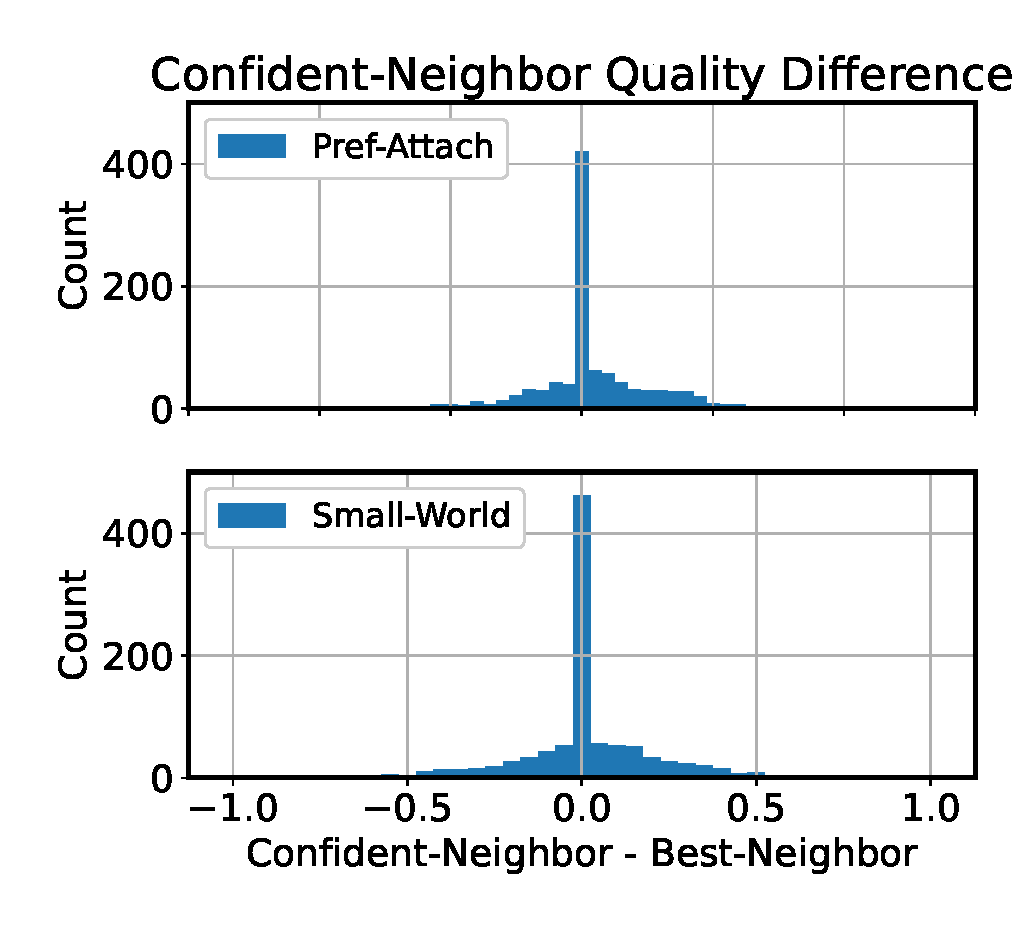
\includegraphics[width=3.33in]{fig/NetDelibABM/fig-results-confident.eps}
\caption{Histograms of the difference in solution quality between confident-neighbor and best-neighbor for both conventional networks.
Results are shown for parallel individual learning.}
\end{figure}

As with conform, the confident-neighbor strategy can be used when available information is insufficient to use best-neighbor. Unlike conform, confident-neighbor models weak social influence. The improved performance of confident-neighbor over best-neighbor, despite using less information, can be attributed at least in part to diversity and exploration. Confident neighbor takes significantly longer to converge, suggesting it maintains a diversity of solutions and allows more time to explore new solutions. Our results suggest several interventions with the potential to improve conventional single-group deliberation. In the presence of weak social influence, reducing the amount of information available can counter-intuitively increase performance. Conversely, when information is already limited, performance might be increased by weakening social influence. However, while confident-neighbor can increase the success of conventional deliberation, it performs comparably to network deliberation using the conform strategy, suggesting that when social influence is strong, network deliberation remains preferable.

\section{Discussion}

We have proposed and evaluated a model of mass deliberation based on the observed interlocking network structure of successful mass-deliberative projects.
Our central finding suggests that network deliberation can improve deliberative output in the presence of strong social influence (i.e., the conform strategy).
Individuals rely on social influence for a number of reasons.
Strong social influence can stem from social factors such as trust or social loafing.
Alternatively, social influence can be used to supplement individual skill when it is insufficient for a given task.
We see that a variety of contexts can lead to reliance on social influence.
Empirical evidence suggests the presence of strong social influence in real-world collaborations such as Wikipedia \cite{platt_network_2018} and in lab studies of human collaboration \cite{mason_collaborative_2012, barkoczi_social_2016}.
In the case of weak social influence (i.e., the  best-neighbor and confident-neighbor strategies), we do not observe a significant difference in output quality between network deliberation and conventional single-group deliberation. In all cases, network deliberation performs better than single-group deliberation or comparatively well. 
Our results suggest that network deliberation is both a contributing mechanism to the success of mass-deliberative projects as well as a useful tool for the design of large-scale sociotechnical systems and interventions for existing systems.

How does network deliberation improve collaborative output? In part, the high performance of random-pod network deliberation can be attributed to the high structural efficiency of the resulting network. However, structural efficiency cannot be the complete mechanism. Long-path network deliberation is extremely inefficient, but still outperforms conventional networks in the presence of strong social influence. The additional mechanisms at play remain an open question.

In order to distinguish between the effects of social influence and individual ability, we have introduced the confident-neighbor strategy, which (unlike best-neighbor) assumes the same agent capabilities as the conform strategy (in a critical learning setting).
While not central to our study of network deliberation, our findings regarding the 
confident-neighbor strategy have important implications for the study of social learning in general. 
Our findings show that just as reducing network efficiency can improve solution quality by raising diversity, reducing the available information can improve the performance of greedy learning strategies. Our investigation of confident-neighbor stems from a careful formal analysis of the information required by each strategy. The surprisingly high performance of confident-neighbor shows the importance of isolating social influence from agent ability.

Our work is limited by a number of assumptions, which require further investigation to achieve greater generalizability. We assume a static objective function, while real-world objectives can change with changing external conditions as well as changing individual preferences. We also assume a homogeneous strategy across all agents, which raises questions of how different strategies interact within the same collaboration. We have also assumed that agents are truthful and do not form coalitions outside of the existing network, both assumptions which can be violated in real-world settings.
We have also assumed that agents have access to the full solution string, and that agents incorporate all bits of the string into their quality estimates. Extremely complex real-world tasks might be better-modeled by a collection of sub-tasks, with agents having access to only a subset of the solution string.
Finally, we have limited our study to learning strategies that explore new solutions solely through small mutations of existing solutions. Other potential strategies might generate entirely new solutions, for example, by combining parts of multiple previous solutions. Such generative strategies would add the ability to explore a wider range of solutions. While our work extends the understanding of social learning and collaboration, many questions still remain open for exploration.

Effective mass deliberation is key to realizing the democratizing power of the internet. Our findings suggest that the presence of small and interlocking pods can contribute to the success of mass deliberation, particularly when the topic is complex and social influence is strong. These findings have implications for a range of deliberative contexts: participatory government and budgeting, worker-owned cooperatives, grassroots social movements, and the governance of decentralized systems (e.g., cryptocurrency). By enabling better deliberation at larger scales, we hope this work will contribute to democratizing the governance of large sociotechnical systems, and empowering the individuals impacted by those systems.

